\subsection{Integración en el flujo de trabajo}
La integración de nuevas personas a un grupo de trabajo es fundamental
dentro de una empresa. Cuando se añaden nuevos miembros, es natural que 
surja cierta fricción debido a diversos factores, como la adaptación a 
la dinámica del equipo, la comprensión de los procesos establecidos y la 
familiarización con las herramientas y tecnologías utilizadas. Esta fricción 
puede ralentizar el progreso del equipo.\medskip

Una forma efectiva de mejorar esta cuestión es mediante la automatización de 
procesos, como la instalación y configuración de herramientas y software necesarios 
para el trabajo del equipo. Al utilizar un script que realiza estas tareas de 
forma automática, se eliminan los posibles errores humanos y se agiliza el proceso 
de integración de los nuevos miembros. Además, al estandarizar la configuración, 
se garantiza que todos los miembros del equipo tengan el mismo entorno de trabajo, 
lo que facilita la compatibilidad. Otro beneficio es que este script puede ser
también utilizado por miembros actuales del equipo para actualizar su entorno de
trabajo actual a las últimas versiones de las herramientas y software utilizados.


\subsubsection{Proceso de integración}
Cuando se incorpora un nuevo miembro al equipo, existe una hoja de ruta que está
definida para que este se acomode lo más rápido posible a la forma de trabajar del
equipo. A continuación se describen los pasos que se siguen para la integración de
un nuevo miembro al equipo:
\begin{enumerate}
    \item \textbf{Pre-requisitos:} antes de comenzar con la integración, es necesario
    que el nuevo miembro tenga a su disposición el ordenador de trabajo con las
    credenciales de acceso a su cuenta de usuario y al servicio de verificación en
    dos pasos.
    \item \textbf{Instalación de herramientas:} el nuevo miembro deberá ejecutar el
    script de instalación de herramientas que se encuentra disponible en la propia
    guía de \textit{Instalación de herramientas}. Este script se encargará de instalar
    todas las herramientas necesarias para el desarrollo de proyectos, aunque por
    razones de seguridad, no se automatizará la creación de ninguna credencial para
    servicios de terceros. Para consultar que herramientas se instalan se pueden ver
    dentro de la sección \textit{Herramientas de desarrollo}.
    \item \textbf{Configuración de autenticación:} aunque las configuraciones básicas
    de las herramientas se han automatizado, es necesario que el nuevo miembro configure
    ciertas credenciales de acceso como la clave ssh de Git-Lab, el token de acceso para ClearML
    y cualquiera otra credencial que sea necesaria para el desarrollo de proyectos.
    \item \textbf{Formación:} una vez que el nuevo miembro ha instalado las herramientas
    y configurado las credenciales, se le proporciona una formación básica sobre el uso
    de dichas herramientas y sobre como implementarlas en su flujo de trabajo.
\end{enumerate}

Con estas directrices, se garantiza que el nuevo miembro pueda comenzar a trabajar
en el menor tiempo posible sin requerir de una ayuda constante por parte de los
miembros actuales del equipo. Una vez terminada la formación, el nuevo miembro
debe haber adquirido las siguientes competencias: uso del sistema de plantillas y componentes,
conocimiento básico de las herramientas de desarrollo, cocimiento básico de la infraestructura,
cocimiento sobre como contribuir en proyectos y en el sistema de conocimiento.

\subsubsection{Herramientas de desarrollo}
A continuación se describen las herramientas que se encuentran dentro del marco
de trabajo del equipo:
\begin{itemize}
    \item \textbf{Python3.11:} se ha elegido la versión 3.11 de Python como versión
    principal para el desarrollo de proyectos. La 3.11 ha traído mejoras significativas
    en cuanto a rendimiento y nuevas funcionalidades sobre la librería estándar como
    el módulo \textit{tomlib} que facilita de la lectura de los toml. Esta versión
    de python es el paquete del repositorio de DeadSnakes, no se utiliza conda ya
    que requiere de una licencia para su uso y no trae ventajas frente a la base.
    \item \textbf{Docker:} debido a que en la actualidad muchos proyectos han de funcionar
    dentro de contenedores, se ha decidido incluir Docker como una de las herramientas por
    dos razones, dar soporte a la virtualización de ciertos proyectos y facilitar su instalación
    que puede llegar a ser complicada si no se tiene experiencia previa.
    \item \textbf{Pipx:} es una herramienta que permite instalar otras herramientas de 
    consola de python de forma aislada, evitando así conflictos entre las distintas 
    versiones de las librerías.
    \item \textbf{Poetry:} es un gestor de dependencias y empaquetador de proyectos de python.
    Se ha incorporado ya que el desarrollo de componentes requiere de una forma sencilla de
    publicar y gestionar las dependencias de cada proyecto. Existe también alternativas como
    Pipenv, pero se ha preferido Poetry por que permite gestionar repositorios privados de una
    forma mas sencilla.  
    \item \textbf{Cookiecutter:} es una herramienta que permite la creación de proyectos a partir
    de plantillas predefinidas. 
    \item \textbf{Ruff:} es una herramienta que se encarga de corregir los errores de estilo
    y formatear el código fuente. Se ha elegido Ruff por encima de otras herramientas como
    Black o Flake8 debido a que Ruff ya combina las funcionalidades de ambas herramientas. Además,
    al estar escrita en rust es mucho más rápida que las otras herramientas. Se puede ver en la 
    figura \ref{fig:ruff-perfor} una comparativa de rendimiento \cite{astralRuff} sobre el repositorio de CPython.
    \begin{figure}[ht]
        \centering
        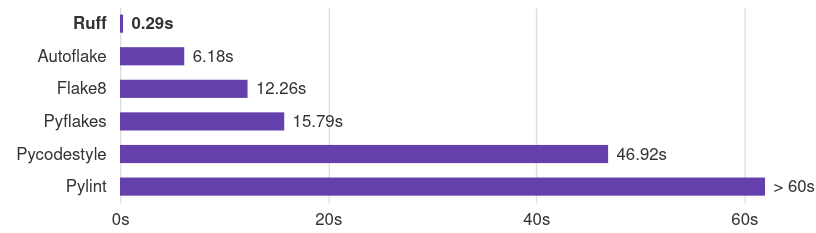
\includegraphics[width=0.8\textwidth]{ruff-perfor.png}
        \caption{Comparativa de rendimiento sobre el repositorio de CPython}\label{fig:ruff-perfor}
    \end{figure}
    \item \textbf{Visual Studio Code:} VSCode es el editor de código mayoritariamente utilizado
    en el mercado tecnológico. Su integración con Python y Docker, así como su facilidad de uso
    y la gran cantidad de extensiones disponibles, lo convierten en una herramienta ideal para
    el desarrollo de proyectos. Se ha elegido VSCode por encima de otras herramientas como PyCharm
    debido a que es más ligero y a diferencia de PyCharm, no requiere de una licencia para su uso.
\end{itemize}


%% TODO: Añadir sección estándares de calidad